% !TeX root = ../../main.tex
\section{Process description}

Nitroma's process for the nitration of toluene and subsequent reduction and hydrogenation of nitrotoluenes is unique in both its continuous operating mode and the production of three different substituted aromatic amines.  \Cref{fig:routes-SI} is a summary of the synthesis routes selected by for Nitroma's process.
\begin{figure}[H]
    \centering
    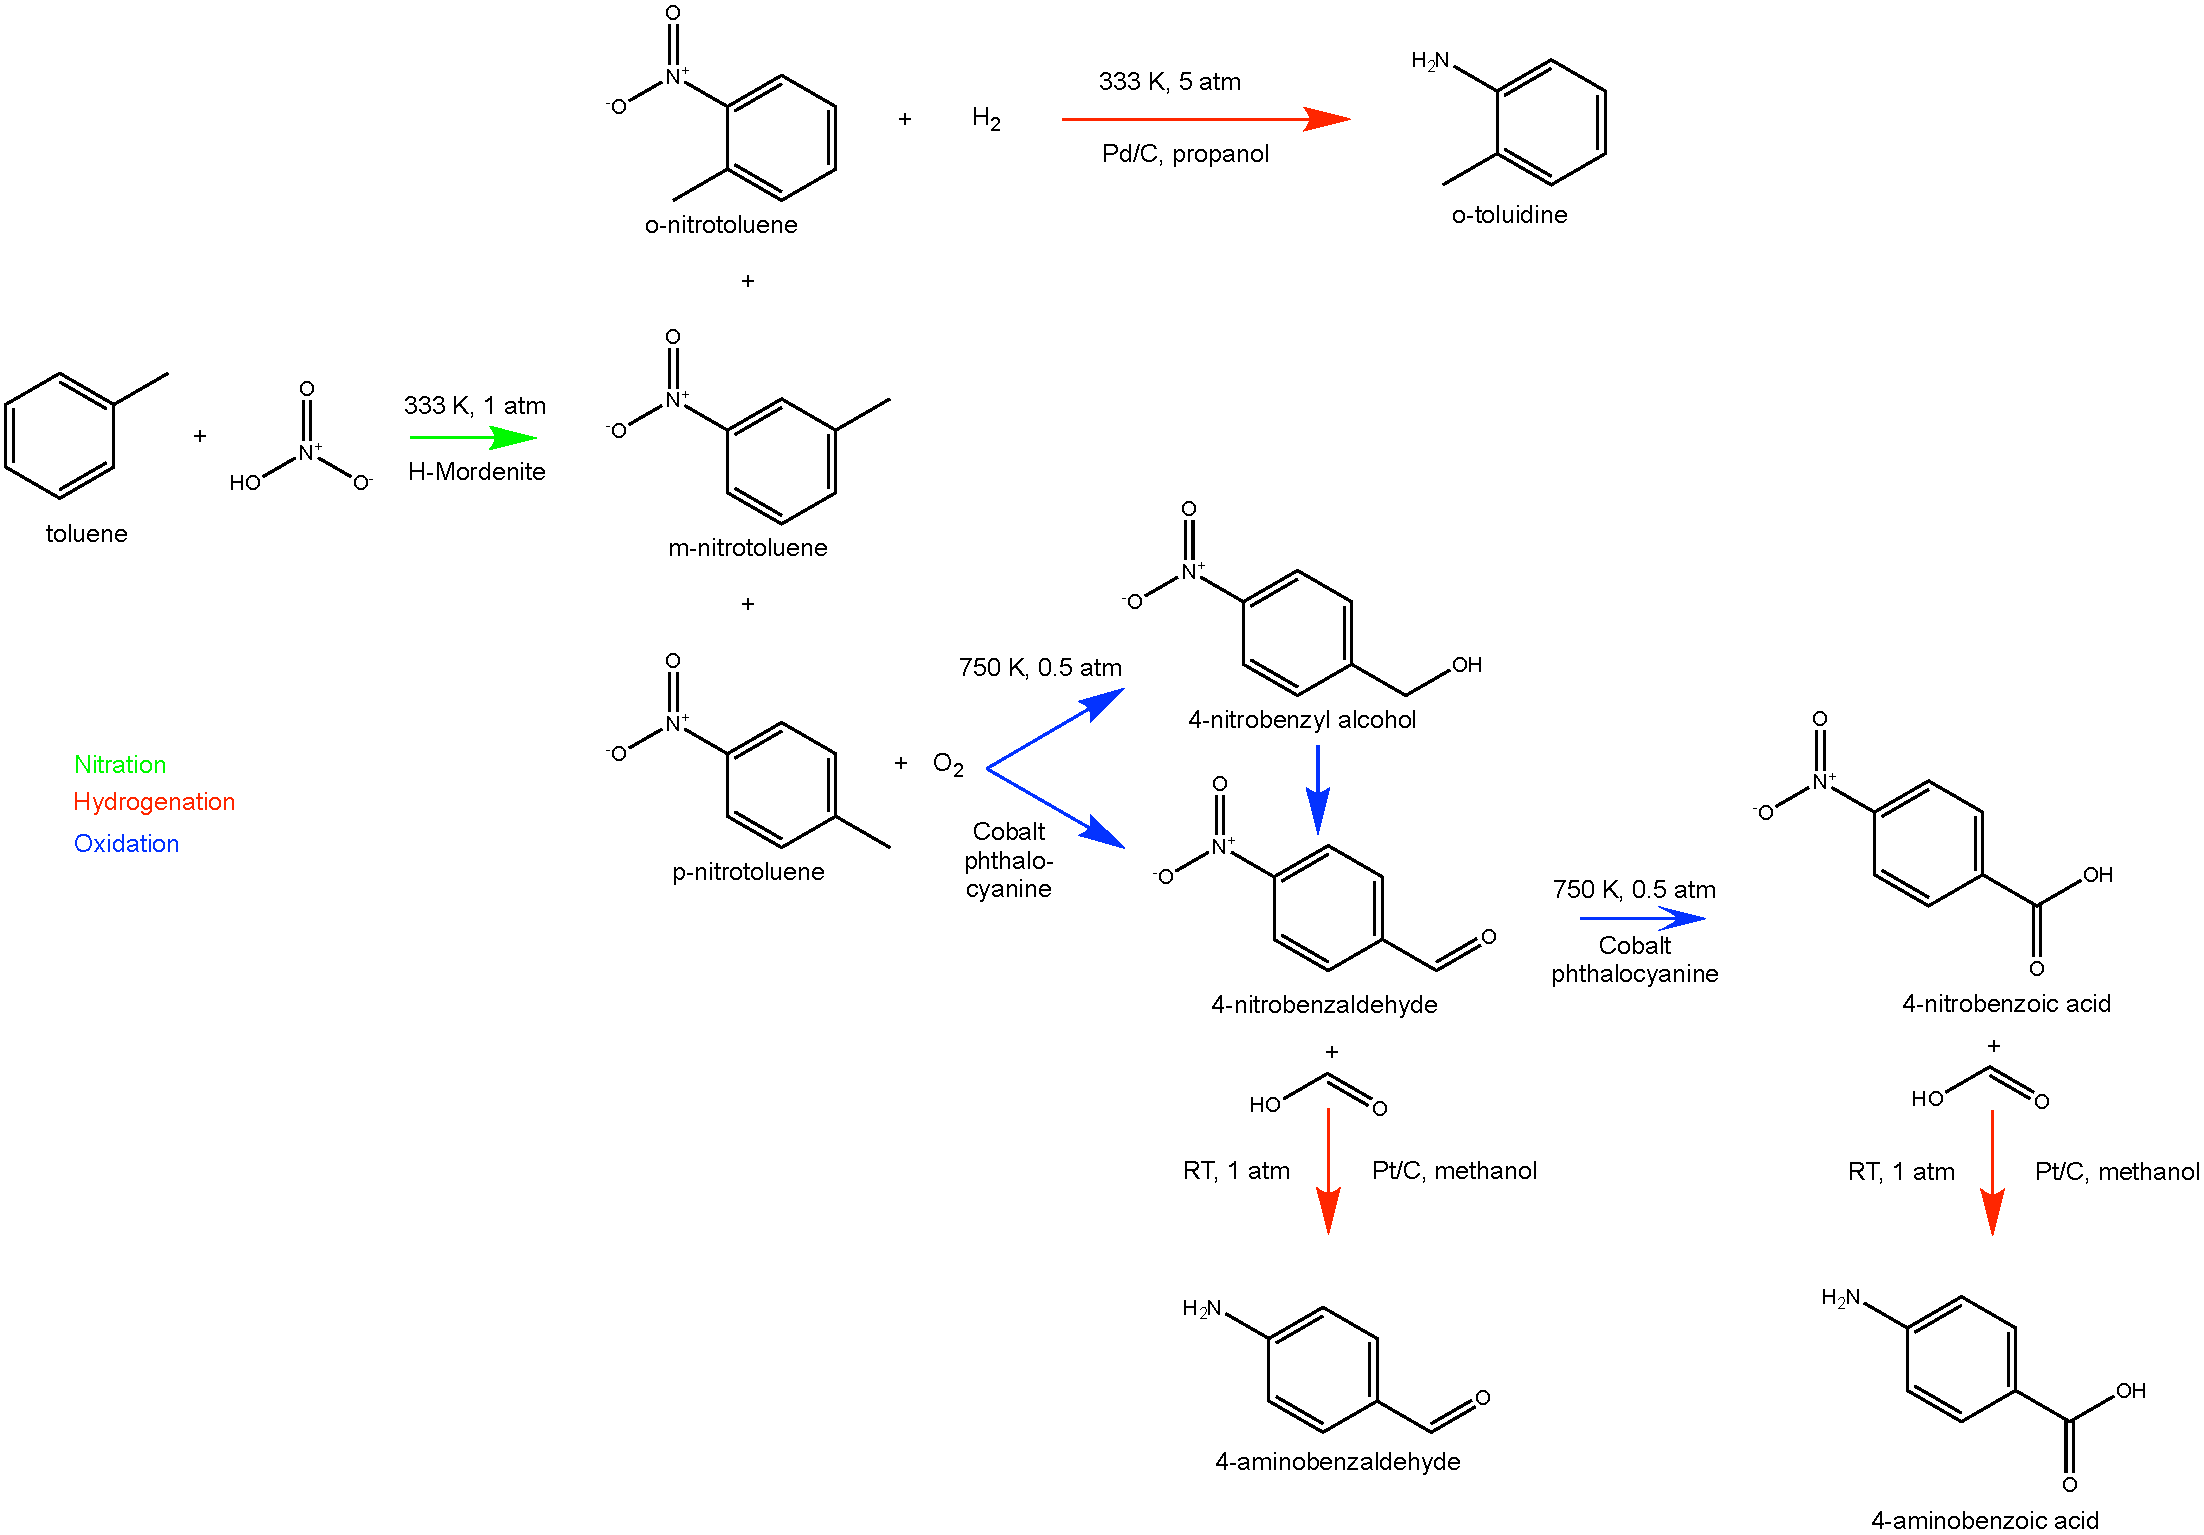
\includegraphics[width=0.8\linewidth]{chapters/1-synthesis/1-Figures/routes-chosen.pdf}
    \caption{Synthesis route for Nitroma's process}
    \label{fig:routes-SI}
\end{figure}

Firstly, the nitration of toluene with 70\% aqueous nitric acid is carried out in a shell-and-tube heat exchanger reactor (R101) packed with H-mordenite catalyst. 1670 tonnes per year of 95\% pure liquid toluene is mixed (M101) with nitric acid in a 1:2 molar ratio. The reaction takes place at atmospheric pressure and the temperature is controlled to stay between 325 and 360K thanks to an innovative cooling system integrated to the reactor. Conversions above 98\% can thus be achieved. The solid acid catalyst and the reaction condition favour the more economically desirable \para-nitrotoluene (PNT) isomer. The nitration reactor effluent is fed to a decanter (S101) to separate the aqueous nitric acid from the organic phase. Following water evaporation in a distillation column (S105), nitric acid is recycled back into the nitration reactor at a \SI{99.8}{mol\percent} purity.  Meanwhile, the organic phase is sent to a distillation column (S102) to recycle unreacted toluene to the nitration reactor. The nitrotoluenes are sent to a second distillation column (S103) to separate the more volatile o-nitrotoluene (ONT) from m-nitrotoluene (MNT) and PNT. The large difference in the PNT and MNT melting points is exploited in a mixed-suspension mixed-product removal crystalliser (S104). The solid PNT crystals are then melt in a hydraulic wash column (S106).

Liquid ONT is mixed with methanol (M201) and hydrogenated under pressure over Pd/C catalyst to o-toluidine (o-TOL) in a co-current trickle bed reactor operating with both gas and liquid in downflow mode. Trickle bed reactor (R201) is chosen due to the ease of operation at high pressure and the relative slow catalyst deactivation. o-TOL is then purified to achieved a purity of \SI{99.4}{mol\percent}. The hydrogen gas leaves the reactor via an outlet port, and the effluent enters a distillation column (S201) to separate methanol and water from the less volatile organic compounds. Methanol is further distilled (S203) to be recycled to the reactor. 

Meanwhile, gaseous PNT is fed into an air-oxidation reactor packed with cobalt phthalocyanine catalyst to be partially oxidised to 4-nitrobenzaldehyde (4-NBH). Depending on the production campaign, the reactor effluent can either be sent to a second oxidation reactor where 4-NBH and unreacted PNT will be completely oxidised to 4-nitrobenzoic acid (4-NBA), owing to longer residence times; or directly to a liquid-phase hydrogenation reactor. Ultimately, 4-NBH and 4-NBA are both reduced to respectively 4-aminobenzaldehyde (4-ABH) and 4-aminobenzoic acid (4-ABA) with formic acid diluted in a methanol solvent over Pt/C catalyst. 4-ABH is purified via a sequence of distillation packed columns whereas 4-ABA is recovered as a solid following  crystallisation in a continuous falling-film melt crystalliser.

 To meet the current customer demand, the plant must operate a 240-day 4-aminobenzaldehyde campaign and a 35-day 4-aminobenzoic acid campain, thus yielding 652 tonnes/year of 99\% pure o-toluidine, 538 tonnes/year of 99.3\% pure 4-aminobenzaldehyde and 100 tonnes/year of pure 4-aminobenzoic acid.